%\documentclass[12pt,a4paper,twoside,draft]{report}
\documentclass[12pt, a4paper]{report}
\usepackage[T2A]{fontenc}
\usepackage[utf8]{inputenc}

\usepackage[main=russian,english]{babel}
\usepackage{amssymb}
\usepackage{amsmath}
\usepackage{amsthm}
\usepackage{epsfig}
\usepackage{array}
\usepackage{longtable}
\usepackage{tabularx}
\usepackage{subfigure}
\usepackage{fancyheadings}
\usepackage{ccfonts}
\usepackage{psfrag}
\usepackage{cite}
\usepackage{euscript}
\usepackage{graphicx}
\usepackage{wrapfig}
\usepackage{epstopdf}
\usepackage[rflt]{floatflt}
\usepackage{floatrow}

\sloppy
\pagestyle{plain}

\newcounter{TaskNumber}
\setcounter{TaskNumber}{1}

\renewcommand{\thesection}{\arabic{section}.}
\renewcommand{\thesubsection}{\arabic{section}.\arabic{subsection}}

% Определяем недостоющие операторы
\DeclareMathOperator*{\argmin}{argmin}
\DeclareMathOperator*{\Argmin}{Argmin}

\theoremstyle{definition}
\newtheorem*{Definition}{Определение}
\theoremstyle{plain}
\newtheorem*{Theorem}{Теорема}
\newtheorem*{Lemma}{Лемма}
\theoremstyle{remark}
\newtheorem*{Remark}{Замечание}
\newtheorem*{Example}{Пример}
\newtheorem*{Consequence}{Следствие}
\theoremstyle{remark}
\newtheorem*{Task}{Задание}
\theoremstyle{definition}
\newtheorem*{ProblemStatement}{Постановка задачи}

\addto\captionsenglish{ \renewcommand*\contentsname{Содержание}}
\addto\captionsenglish{\renewcommand{\figurename}{Рис.}}
\addto\captionsrussian{\def\refname{Список используемой литературы}}


\author{Zavgorodniy Igor, 442}
\title{Отчёт}
\date{}

%\includeonly{Title,0-Introduction,Ch1,Ch2,Ch3,Conclusion,Bibliography}


\begin{document}
\begin{titlepage}
  \begin{center}
    \large
   ФЕДЕРАЛЬНОЕ ГОСУДАРСТВЕННОЕ БЮДЖЕТНОЕ ОБРАЗОВАТЕЛЬНОЕ УЧРЕЖДЕНИЕ\\ ВЫСШЕГО ОБРАЗОВАНИЯ\\ "МОСКОВСКИЙ ГОСУДАРСТВЕННЫЙ УНИВЕРСИТЕТ\\ имени М.В.ЛОМОНОСОВА''\\
    ФИЗИЧЕСКИЙ ФАКУЛЬТЕТ\\КАФЕДРА ФИЗИКО-МАТЕМАТИЧЕСКИХ МЕТОДОВ УПРАВЛЕНИЯ

	\underline{\hspace{12cm}}

    \vfill

    {\LARGE \textbf{Выпускная дипломная работа}}
  	\bigskip
  	
    {\textbf{Обучение с подкреплением\\ в задаче поиска пути в лабиринте}}  	
  	\bigskip


\end{center}
\vfill

\begin{flushright}
Выполнил студент IV курса:\\
Завгородний Игорь Викторович\\
\bigskip
Научный руководитель:\\
Галяев А.А.
%$\labda$
\end{flushright}
\vfill

\begin{center}
  Москва\\2019
\end{center}
\end{titlepage}

\newpage
\section{Введение}
Данная работа посвящена применению метода обучения с подкреплением (Reinforcement Learning) в задаче поиска оптимального пути в трёхмерном лабиринте. Построеннаые математические и програмные модели применимы для описания движения агентов в различных физических системах. Например, описание движения беспилотного летательного аппарата (БПЛА), выполняющего задачи в различных слоях атмосферы, описание движения автономного подводного судна, выполнящего исследования на разной глубине, и так далее.

В результате работы был создан и протестирован алгоритм, позволяющий осуществлять оптимальное управление агентом в трёхмерном лабиринте, имитирующим атмосферу. Метод обучения с подкреплением показал эффективность при обучении агента на заданных лабиринтах, где данные не меняются с течением времени, что, безусловно, отличается от реальных процессов.

\newpage
\tableofcontents

\newpage
\section{Теоретическое введение}
\label{sec:W1}
Современные задачи науки и техники требуют применения современных методов, позволяющих быстро и корректно обратывать большие объёмы данных, ежесекундно поступающих с многочисленных датчиков. Более того, с увеличением объёма задач, стоящих перед кибернетическии агентами, усложняется их поведение. Традиционные методы программирования исчерпывают себя, делая решение современных задач неэффективным по затрачиваемому времени и используемой памяти.\\

Данные проблемы призван преодолеть метод машинного обучения (Machine Learning), фундаментальные основы которого были заложены еще в 1940-1950-х годах прошлого века. Однако бурное развитие подобных методов началось лишь в 1990-х годах вместе с ростом вычислительных мощностей компьютеров.
Достоинством данного метода является отсутсвие необходимости создавать детерменированные алогритмы, полностью покрывающие необходимые сценарии поведения агентов. Машинное обучение позволяет создать агентов нового типа, способных обучаться и строить оптимальные алгоритмы при минимальном воздействии человека.\\

Существует две основных концепции машинного обучения: обучение с учителем, в котором агент обучается производить определённые действия на основании предварительно подготовленных выборок, и обучение без учителя, в котором агент самостоятельно формирует стратегию поведения, опираясь на изменения, производимые его действиями. Обучение с подкреплением принадлежит ко второму типу машинного обучения. Агент перебирает все варианты действий и из всех возможных действий выбирает те, которые принесут ему наибольшее итоговое вознаграждение. Перечисленные концепции называются "методом проб и ошибок" и "отсроченным поощрением"\, они лежат в основе обучения с подкреплением.\\

В данной работе для решения задачи поиска пути в лабиринте применяется метод обучения с подкреплением. Как было сказано ранее, одной из особенностей метода является то, что обучение агента происходит благодаря взаимодействию с окружающей средой. Лабиринт - это и есть среда, предназначенная для экспериментального исследования, в которой движется управляемый агент. Задача поиска пути в лабиринте является одной из ключевых задач в робототехнике, решение которой позволяет создавать системы управления движением автономных роботов (дронов). \\

Метод обучения с подкреплением в общем виде можно представить в качестве марковского процесса принятия решений:
\begin{center}
	 $ (S, A, P_a(s, s'), R_a(s, s')),$ где:
\end{center}
\begin{enumerate}
 	\item $S$ - множество возможных состояний среды,
 	\item $A$ - множество возможных действий агента над средой,
 	\item $P_a(s, s') = P(s_{t+1}=s'\,|\,s_t=s,\:a_t=a)$ - вероятность, что состояние $s$ под действием $a$ во время $t$ перейдёт в состояние $s'$ ко времени $t+1$,
 	\item $R_a(s, s') = R(s_{t+1}=s'\,|\,s_t=s,\:a_t=a)$ - вознаграждение, получаемое после перехода в состояние $s'$ из состояния $s$ с вероятностью $P_a(s,s')$.
\end{enumerate}


Поведение агента описывается следующей цепочкой действий:
\begin{center}
состояние $\rightarrow$ действие
$\rightarrow$ поощрение $\rightarrow$ состояние $\rightarrow$ \\
$\rightarrow$ действие $\rightarrow$ поощрение $\rightarrow$ ... 
\end{center}

\begin{figure}[h]
	\center{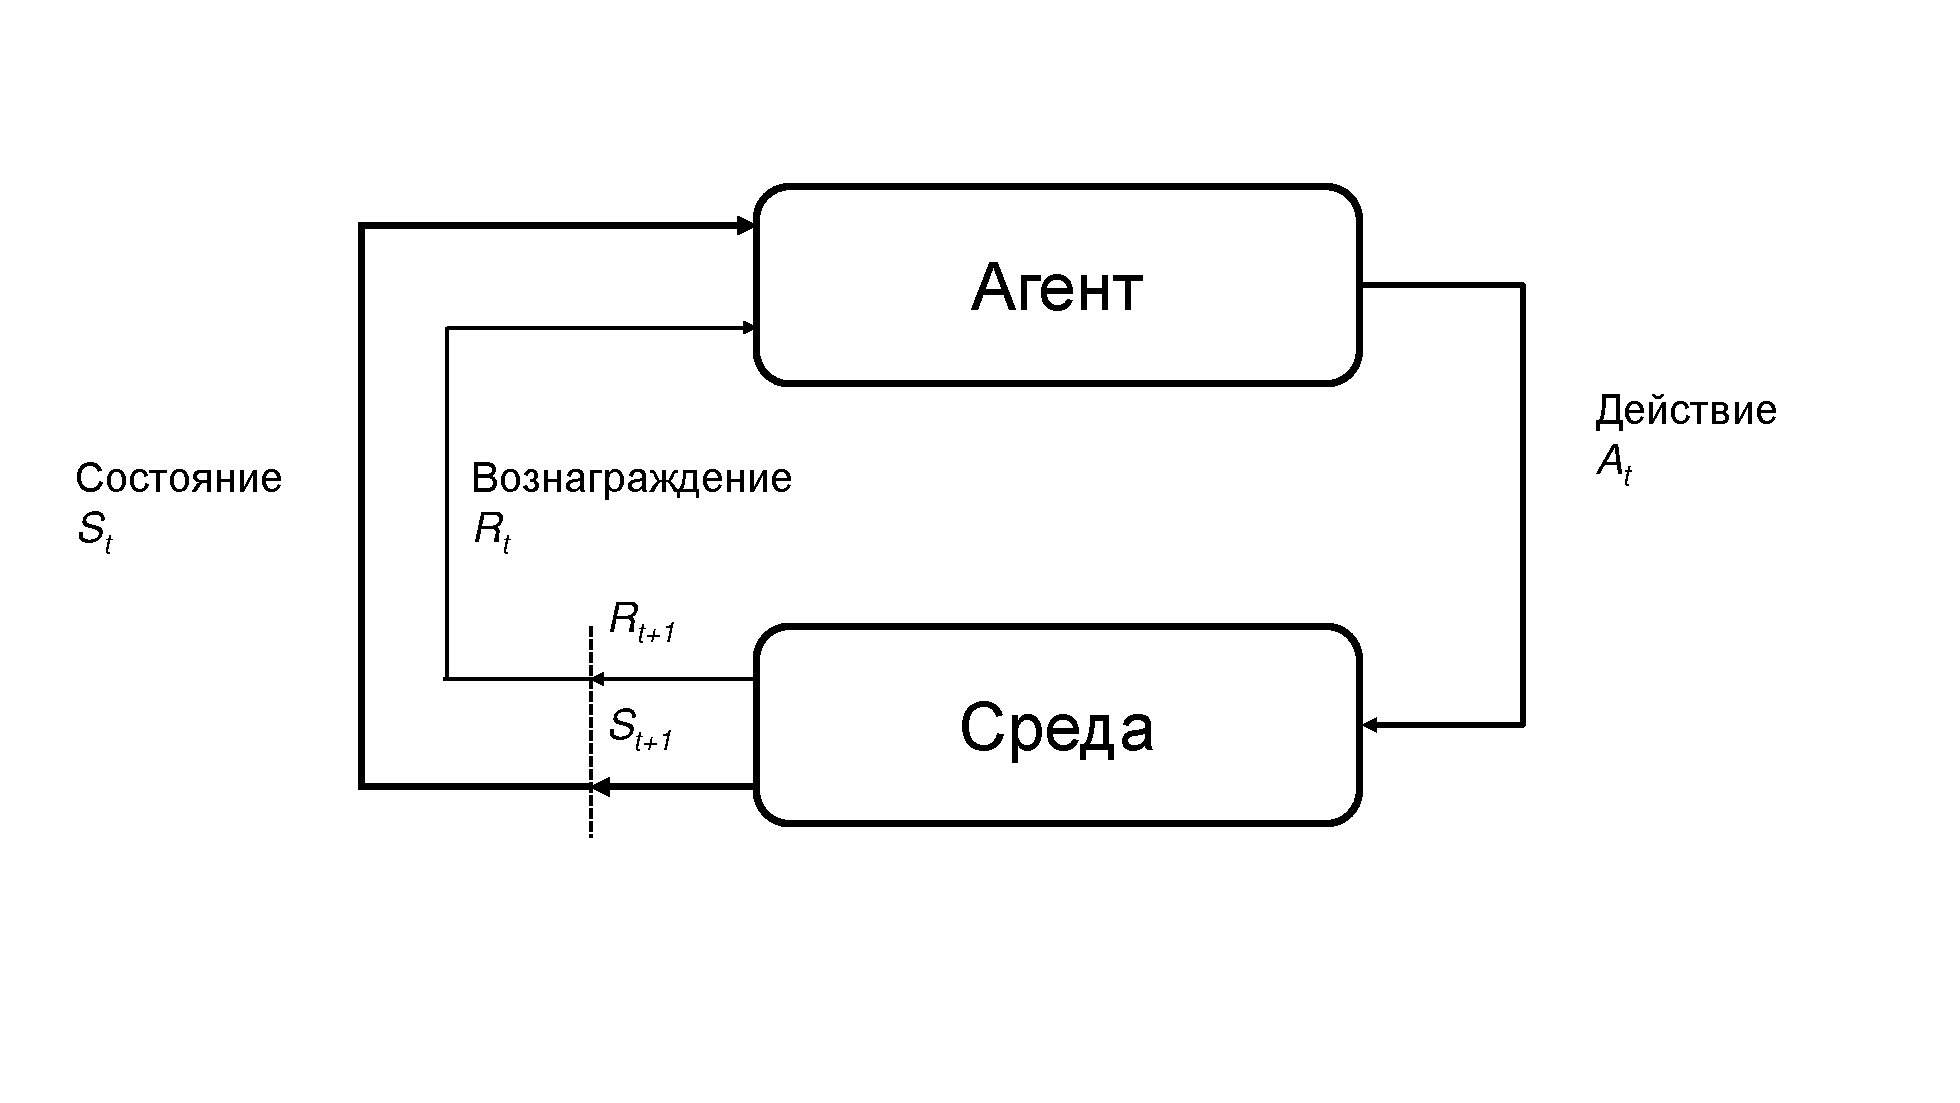
\includegraphics[scale = 0.25]{SARSA.pdf}}
	\caption{SARSA-модель}
\end{figure}

В англоязычной литературе данный процесс носит название «SARSA» («State-Action-Reward-State-Action-...»).\\

Вводится некоторая политика (англ. \textit{policy}):
\begin{center}
	$\pi \, : \; S \times A \rightarrow [0, 1]$

$\pi(a\,|\,s) = P(a_t=a\,|\,s_t=s)$ - вероятность действия $a$ в состоянии $s$.
\end{center}

Цель агента - выбрать такую оптимальную политику $\pi$, обозначающую вероятность выбора действия $a$ в состоянии $s$, чтобы при следовании ей сумма вознаграждений, получаемых от среды, была максимальна.
Ожидаемая награда в момент времени $t$ определяется как:

$$R_t = E[r_t \,+\, \gamma r_{t+1} \,+\, \gamma^2 r_{t+2}\, +\,\, ...] = E\left[\sum_{k=0}^{\infty}\gamma^kr_{t+k}\right],$$

где $E[\cdot]$ - математическое ожидание, $\gamma\in(0, 1)$ - коэффициент дисконтирования (англ. \textit{discount rate}).

Долгосрочная стратегия агента в общем случае не подразумевает преследование максимальной выгоды на каждом ромежуточном шаге. Непосредственный выбор стратегии может осуществляться множеством способов.
Введем функцию $Q(s,a)$ , которая парам состояние-действие ставит в соотвествие число. Данное число называется ценностью состояния-действия. Также на каждом временном шаге $ t $ агент получает вознаграждение $ r_{t} $:

$$Q^{\pi}(s, a) = E_{\pi}[R_t|\,s_t=s, a_t=a] = E_{\pi}\left[\sum_{k=0}^{\infty}\gamma^kr_{t+k}\,|\,s_t=s, a_t=a\right],$$

где индекс $\pi$ означает выбор действий в соотвествии с некоторой политикой (\textit{policy}).\\

Эта функция характеризует ожидаемую награду, получаемую агентом стартуя из состояния $s, s \in S$ совершая действие $a, a \in A$, и в дальнейшем действуя в соответсвии с определенной политикой $\pi$.

Отсюда мы можем получить рекурсивную формулу для оценки данной функции:\\

\begin{center}
	$Q_{i+1}^{\pi}(s, a) = E_{\pi}\left[r_t + \gamma\sum_{k=0}^{\infty}\gamma^kr_{t+k+1}\,|\,s_t=s, a_t=a\right] = E_{\pi}\left[r_t + \gamma Q_{i}^{\pi}(s_{t+1}=s', a_{t+1}=a')\,|\,s_t=s, a_t=a\right]$
\end{center}

Однако целью агента является - нахождение оптимальной политики $\pi$, на которой достигается максимальная ожидаемая награда. Таким образом, мы должны найти такую $\pi^*$, которая в результате нам дает максимальное значение action-value функции $Q^*(s, a)$ среди всех существующих политик. Формула для оценки оптимального значения action-value функции определяется следующим образом:
$$Q_{i+1}(s, a) = E[r_t + \gamma max_{a'}Q_i(s', a')\,|\,s, a]$$

При $i \rightarrow \infty$ следует, что $Q_{i}(s, a) \rightarrow Q^*(s, a)$. Данный процесс называется \textit{алгоритмом итерации значений} (англ. \textit{value iteration algorithm}).

\section{Постановка и формализация задачи}

\begin{figure}[h]
	{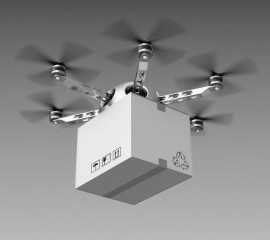
\includegraphics[scale = 0.6]{dronebw.jpg}}
	\caption{Беспилотный аппарат}
\end{figure}

Рассмотрим движение беспилотного аппарата (агента) в атмосфере (испытательной среде, лабиринте). Задачей агента является сбор грузов в различных точках пространтва и их доставка до точек выгрузки с наименьшими затратами топлива.\\

Для описания системы используются следующие величины:
\begin{enumerate}
	\item $\vec{r}\ (x,y,z)$ - координата беспилотного аппарата в трёхмерном пространстве: $x\in[0; l_{x}]$, $y\in[0; l_{y}]$, $z\in[0; l_{z}]$;
	\item $\rho (\vec{r})$ - плотность атмосферы в точке пространства:  $\rho \in[\rho_{min}; \rho_{max}]$;
	\item $F$ - статус наличия груза: $F \in \lbrace 0; 1\rbrace$.
\end{enumerate}

Множество действий, доступных агентов состоит из восьми элементов:
\begin{enumerate}
	\item Движение на Юг (south);
	\item Движение на Север (north);
	\item Движение на Восток (east);
	\item Движение на Запад (west);	
	\item Движение на Вверх (east);
	\item Движение на Вниз (west);
	\item Сбор груза (pickup);
	\item Сброс груза (dropoff);	
\end{enumerate}

Таким образом, состояние среды описывается четыремя непрерывными вещественными числами, а множество действий состоит из двух значений.


Беспилотный аппарат (агент) движется в трёхмерном пространстве(среда), каждому слою атмосферы соотвествует одна координата по оси Z, с каждым слоем уменьшается общий для слоя мультипликатор. Кроме того, каждому слою атмосферы соответсвует определённое распределение плотности воздуха по осям Х и У, реализованное случайной расстановкой очков вознаграждения.

\section{Описание используемых методов}

Перед тем как описывать способы определения ценностей для пар состояний-действий, стоит указать используемые стратегии выбора действий. В данной задаче есть два принципиально разных класса состояний, следовательно, и стратегии для них тоже должны быть разные. В случае, когда производится выбор карты для озвучивания, карта выбирается следующим образом. В руке находятся наименования с наибольшим количеством карт,
далее из них случайно выбирается одно наименование. Во втором случае используется -жадная стратегия, она заключается в жадном выборе действия (действие, которое максимизируетQ(s, a)  с вероятностью , в остальных случаях действие выбирается случайно. Все используемые в работе методы построения оценки функции ценности пар состояний-действий основаны на методе временных различий (TD — Temporal-Difference). В TD-методах процесс обучения основывается на опыте взаимодействия агента со средой без использования модели среды. Расчетные оценки состояний (в случае задачи управления состояний-действий) в TD-методах обновляются, основываясь на других полученных оценках, т.е. они самонастраиваются [2]. Классический TD-метод используют для построения оценок ценности состояния среды. Опишем его, перед тем как перейти к случаю управления. В данной работе будут использоваться идеи многошагового TD-метода, так же известного как метод TD, и одношагового метода, или метода TD(0), который является частным случаем многошагового. В многошаговом методе имеется переменная памяти e(s) , соответствующая каждому состоянию. Она называется следом приемлемости [2]. На каждом временном шаге следы приемлемости для всех состояний, кроме текущего, убывают с коэффициентом, а след приемлемости для посещаемого на данном шаге состояния увеличивается на параметр затухания следа,  — коэффициент приведения. След приемлемости все время регистрирует, посещение каких состояний имело место недавно, где смысл понятия "недавно" определяется с помощью коэффициента. Процесс оценки состояний проходит следующим образом. Во время обучения при переходе из состояний st в состояние st+1 вычисляется величина 
где V(st) — функция ценности состояния, аналогичная функции ценности пар состояний-действий Q(s, a) . Далее для всех состояний производится корректировка их ценности с использованием следов приемлемости где — коэффициент обучения. Соответственно, в случае одношагового метода никаких следов приемлемости нет, т.к.  = 0 , поэтому на каждом шаге производится только корректировка ценности состояния st, что можно записать в виде
Одним из наиболее важных достижений в обучении с подкреплением стало развитие управления по TD-методу с разделенной оценкой ценности стратегий, известного как Q-обучение. В данной работе используется простейший одношаговый алгоритм корректировки ценностей пар состояние- действие, который основывается на одношаговом методе TD, (4) с штрихами здесь состояния и действия$ st+1 иat+1 $ , без штрихов stиat . В этом случае искомая функция ценности действия Q непосредственно аппроксимирует оптимальную функцию ценности действий, независимо от применяющейся стратегии. [3].
Альтернативой методам Q-обучения является метод SARSA (State-Action- Reward-State-Action), который основывается на модели обобщенной итерации по стратегиям с использованием TD-метода в оценочной или предсказательной
части. В данной работе используется TD-метод управления с интегрированной оценкой ценности стратегий. Последовательность действий в методе SARSA() базируется на двух шагах. Первый шаг заключается в изучении функции ценности действий. Для этого необходимо оценить функцию Q(s, a) для состояния s и всех действий a. Далее выбирается действие a и производится переход в следующее состояние. Второй шаг повторяет первый, только в конце
шага вместо перехода производится корректировка ценностей всех пар состояний-действий [4]. По аналогии с методом TD() находится величина, а далее для всех пар состояний-действий производится корректировка оценок и корректировка всех следов приемлемости.

\section{Программная реализация}
Основой для решения послужила библиотека Gym от OpenAI. Библиотека содержала, рассмотренную мной задачу в упрощённом виде: обучение с подкреплением использовалось для оптимизации обработки заказов и движения такси в двумерном лабиринте.\\
Несмотря на кажущуюся схожесть с задачей управления беспилотным аппаратом, требовалась серьёзная доработка существующего решения:
\begin{itemize}
\item Требовалось обощить задачу на случай движения в трёх измерениях;
\item Требовалось изменить постановку задачи так, чтобы добавить физический и прикладной смыслы.
 \end{itemize}

Обе задачи были выполнены. 

\section{Результаты работы}
\section{Вывод}
%\begin{itemize}
%\item Удалось синтезировать ПИД-регулятор, удовлетворяющий заданным условиям;
%\item Дополнительное иссоелование системы позволяет говорить об устойчивости системы, достигнутой благодаря синтезу регулятора.
 %\end{itemize}

\newpage
\section{Список используемой литературы} 
$[1]$ Комаров А. Ю., Метод обучения с подкреплением для архитектуры вероятностных автоматов.\\
$[2]$ Князятов С.А., Малинецкий Г.Г.,
Решение задачи распознавания блефа в игре «верю – не верю» с помощью алгоритмов
обучения с подкреплением // Препринты ИПМ им. М.В.Келдыша. 2018. No 170. 21 с.\\
$[3]$ André Barreto, Will Dabney, Rémi Munos, Jonathan J. Hunt,
Tom Schaul, Hado van Hasselt, David Silver, Successor Features for
Transfer in Reinforcement Learning \\
$[4]$ André Barreto, Will Dabney, Rémi Munos, Jonathan J. Hunt,
Tom Schaul, Hado van Hasselt, David Silver, Successor Features for
Transfer in Reinforcement Learning \\
$[5]$ Romain Laroche, Merwan Barlier, Transfer Reinforcement Learning with Shared Dynamics \\
$[6]$ Саттон Р., Барто Э. Обучение с подкреплением – Бином. Лаборатория знаний,
2012. – 400 с.

\end{document} 